\subsection{Manipulationsknoten}

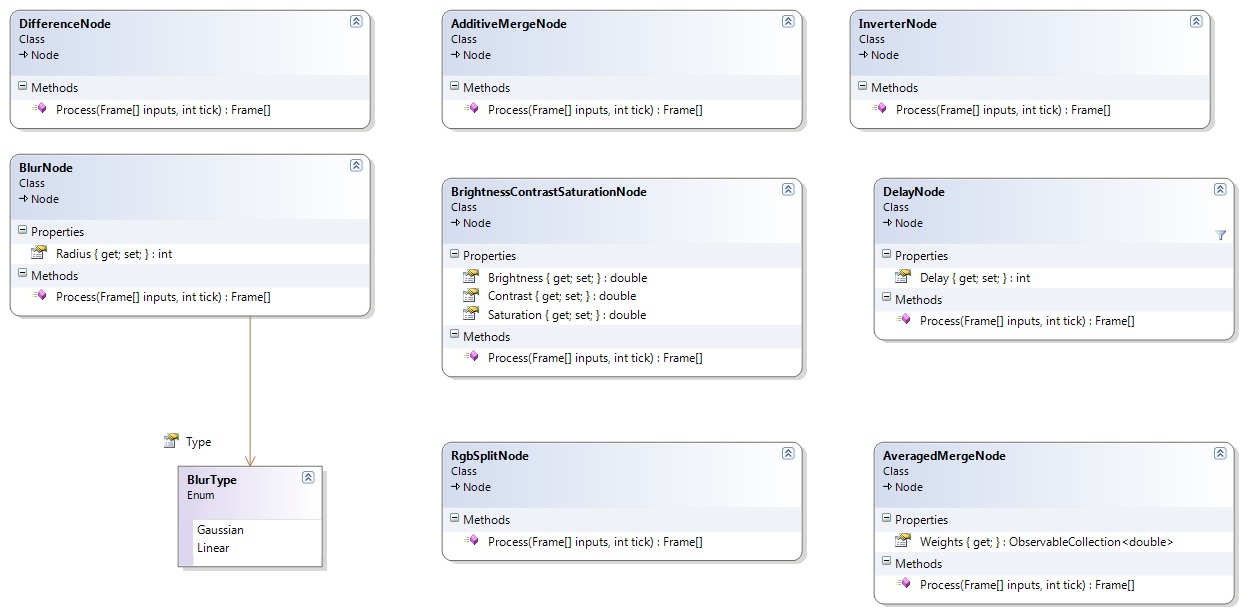
\includegraphics[width=\textwidth]{YuvKA.Pipeline/manipulationnodes.png}
UML-Klassendiagramm der Knoten, die Videostreams innerhalb der Pipeline verändern können.

\subsubsection{YuvKA.Pipeline.InverterNode}

\subsubsection{YuvKA.Pipeline.BlurNode}

\begin{verbatim}
public class BlurNode : Node
\end{verbatim}

\paragraph{Beschreibung}~\\
Die Klasse \name{BlurNode} modelliert die Weichzeichnung der \name{Frame}s des Videos.

\paragraph{Typmember}
\begin{itemize}

\property{Type}
	\begin{verbatim}
	public BlurType Type { get; set; }
	\end{verbatim}
	Ruft die Art der Weichzeichnung ab, oder legt sie fest. Standardmäßig werden gaußsches und lineares Weichzeichnen unterstützt.
	
\property{Radius}
	\begin{verbatim}
	[Range(0.0, double.PositiveInfinity)]
	public int Radius { get; set; }
	\end{verbatim}
	Ruft die den Weichzeichnungsradius ab, oder legt diesen fest. Dieser Wert ist maßgeblich für das Ausmaß der Weichzeichnung.

\method{ProcessFrame}
	\begin{verbatim}
	public override Frame[] ProcessFrame(Frame[] inputs, int frameIndex)
	\end{verbatim}
	Zeichnet den übergebenen \name{Frame} weich. Die genaue Art der Weichzeichnung wird hierbei durch \name{Type} festgelegt. Die standardmäßig unterstützten Arten sind:
	\begin{description}
		\item[Lineares Weichzeichnen]~\\
			Beim linearen Weichzeichnen wird der neue Wert eines Pixels dadurch berechnet, dass die alten Werte aller umliegenden Pixel innerhalb einer Box mit Höhe und Breite (2 * \name{Radius}) + 1 gemittelt werden.~\\
			-insert pseudocode here-
		\item[Gaußsches Weichzeichnen]~\\
			Beim Gaußschen Weichzeichnen wird der neue Wert eines Pixels durch eine gewichtete Mittlung der umliegenden Pixel berechnet. Die Gewichtung der umliegenden Pixel wird hierbei durch folgende gaußsche Funktion definiert:\\
			\[
			G(x,y) = \frac{1}{\sqrt{2\pi\sigma^2}}e^{-\frac{x^2}{2\sigma^2}}
			\]
			Wobei $\sigma$ der \name{Radius} ist.\\
			-insert pseudocode here-
	\end{description}
	
\end{itemize}

\subsubsection{YuvKA.Pipeline.BrightnessContrastSaturationNode}

\subsubsection{YuvKA.Pipeline.AdditiveMergeNode}

\subsubsection{YuvKA.Pipeline.AverageMergeNode}

\begin{verbatim}
public class AveragedMergeNode : Node
\end{verbatim}

\paragraph{Beschreibung}~\\
Die Klasse \name{AverageMergeNode} modelliert das Zusammenführen von Videos durch gewichtete Mittlung der \name{Frame}s.

\paragraph{Typmember}
\begin{itemize}

\property{Weights}
	\begin{verbatim}
		[Range(0.0, 1.0)]
		public ObservableCollection<double> Weights { get; private set; }
	\end{verbatim}
	Ruft eine Sammlung von Gewichtungen einzelner Videos ab, oder legt diese fest.

\method{ProcessFrame}
	\begin{verbatim}
	public override Frame[] ProcessFrame(Frame[] inputs, int frameIndex)
	\end{verbatim}
	Mittelt alle übergebenen \name{Frame}s Pixelweise unter beachtung der von \name{Weights} defienirten Gewichtungen.\\
	-pseudocode notwendig?-
	
	
\end{itemize}

\subsubsection{YuvKA.Pipeline.DifferenceNode}

\subsubsection{YuvKA.Pipeline.DelayNode}

\begin{verbatim}
public class DelayNode : Node
\end{verbatim}

\paragraph{Beschreibung}~\\
Die Klasse \name{DelayNode} modelliert die Verzögerung von Videostreams innerhalb der Pipeline.

\paragraph{Typmember}
\begin{itemize}

\field{Queue}
	\begin{verbatim}
	Queue<Frame> queue
	\end{verbatim}
	Enthält eine Warteschlange von \name{Frame}s die Verzögert werden.
	
\property{Delay}
	\begin{verbatim}
	[Range(0, 10)]
	public int Delay { get; set; }
	\end{verbatim}
	Ruft die Dauer der Verögerung in der Einheit \name{Frame}s ab, oder legt sie fest.

\method{ProcessFrame}
	\begin{verbatim}
	public override Frame[] ProcessFrame(Frame[] inputs, int frameIndex)
	\end{verbatim}
	Stellt den übergebenen \name{Frame} in die Warteschlange \name{Queue} mit der Länge \name{Delay} an, und gibt den ersten \name{Frame} der Warteschlange zurück.
	
\end{itemize}

\subsubsection{YuvKA.Pipeline.RgbSplitNode}

\begin{verbatim}
public class RgbSplitNode : Node
\end{verbatim}

\paragraph{Beschreibung}~\\
Die Klasse \name{RgbSplitNode} modelliert die Aufteilung der \name{Frame}s eines Videos in die Farbkanäle Rot, Grün und Blau.

\paragraph{Typmember}
\begin{itemize}

\method{ProcessFrame}
	\begin{verbatim}
	public override Frame[] ProcessFrame(Frame[] inputs, int frameIndex)
	\end{verbatim}
	Erzeugt aus dem übergebenen \name{Frame} drei neue \name{Frame}s die jeweils nur einen Farbkanal des ursprünglichen \name{Frame}s enthalten und gibt diese drei \name{Frame}s zurück.
	
\end{itemize}